% Options for packages loaded elsewhere
% Options for packages loaded elsewhere
\PassOptionsToPackage{unicode}{hyperref}
\PassOptionsToPackage{hyphens}{url}
%
\documentclass[
  english,
  russian,
  12pt,
  a4paper,
  DIV=11,
  numbers=noendperiod]{scrreprt}
\usepackage{xcolor}
\usepackage{amsmath,amssymb}
\setcounter{secnumdepth}{5}
\usepackage{iftex}
\ifPDFTeX
  \usepackage[T1]{fontenc}
  \usepackage[utf8]{inputenc}
  \usepackage{textcomp} % provide euro and other symbols
\else % if luatex or xetex
  \usepackage{unicode-math} % this also loads fontspec
  \defaultfontfeatures{Scale=MatchLowercase}
  \defaultfontfeatures[\rmfamily]{Ligatures=TeX,Scale=1}
\fi
\usepackage{lmodern}
\ifPDFTeX\else
  % xetex/luatex font selection
  \setmonofont[]{DejaVu Sans Mono}
\fi
% Use upquote if available, for straight quotes in verbatim environments
\IfFileExists{upquote.sty}{\usepackage{upquote}}{}
\IfFileExists{microtype.sty}{% use microtype if available
  \usepackage[]{microtype}
  \UseMicrotypeSet[protrusion]{basicmath} % disable protrusion for tt fonts
}{}
\usepackage{setspace}
% Make \paragraph and \subparagraph free-standing
\makeatletter
\ifx\paragraph\undefined\else
  \let\oldparagraph\paragraph
  \renewcommand{\paragraph}{
    \@ifstar
      \xxxParagraphStar
      \xxxParagraphNoStar
  }
  \newcommand{\xxxParagraphStar}[1]{\oldparagraph*{#1}\mbox{}}
  \newcommand{\xxxParagraphNoStar}[1]{\oldparagraph{#1}\mbox{}}
\fi
\ifx\subparagraph\undefined\else
  \let\oldsubparagraph\subparagraph
  \renewcommand{\subparagraph}{
    \@ifstar
      \xxxSubParagraphStar
      \xxxSubParagraphNoStar
  }
  \newcommand{\xxxSubParagraphStar}[1]{\oldsubparagraph*{#1}\mbox{}}
  \newcommand{\xxxSubParagraphNoStar}[1]{\oldsubparagraph{#1}\mbox{}}
\fi
\makeatother

\usepackage{color}
\usepackage{fancyvrb}
\newcommand{\VerbBar}{|}
\newcommand{\VERB}{\Verb[commandchars=\\\{\}]}
\DefineVerbatimEnvironment{Highlighting}{Verbatim}{commandchars=\\\{\}}
% Add ',fontsize=\small' for more characters per line
\usepackage{framed}
\definecolor{shadecolor}{RGB}{241,243,245}
\newenvironment{Shaded}{\begin{snugshade}}{\end{snugshade}}
\newcommand{\AlertTok}[1]{\textcolor[rgb]{0.68,0.00,0.00}{#1}}
\newcommand{\AnnotationTok}[1]{\textcolor[rgb]{0.37,0.37,0.37}{#1}}
\newcommand{\AttributeTok}[1]{\textcolor[rgb]{0.40,0.45,0.13}{#1}}
\newcommand{\BaseNTok}[1]{\textcolor[rgb]{0.68,0.00,0.00}{#1}}
\newcommand{\BuiltInTok}[1]{\textcolor[rgb]{0.00,0.23,0.31}{#1}}
\newcommand{\CharTok}[1]{\textcolor[rgb]{0.13,0.47,0.30}{#1}}
\newcommand{\CommentTok}[1]{\textcolor[rgb]{0.37,0.37,0.37}{#1}}
\newcommand{\CommentVarTok}[1]{\textcolor[rgb]{0.37,0.37,0.37}{\textit{#1}}}
\newcommand{\ConstantTok}[1]{\textcolor[rgb]{0.56,0.35,0.01}{#1}}
\newcommand{\ControlFlowTok}[1]{\textcolor[rgb]{0.00,0.23,0.31}{\textbf{#1}}}
\newcommand{\DataTypeTok}[1]{\textcolor[rgb]{0.68,0.00,0.00}{#1}}
\newcommand{\DecValTok}[1]{\textcolor[rgb]{0.68,0.00,0.00}{#1}}
\newcommand{\DocumentationTok}[1]{\textcolor[rgb]{0.37,0.37,0.37}{\textit{#1}}}
\newcommand{\ErrorTok}[1]{\textcolor[rgb]{0.68,0.00,0.00}{#1}}
\newcommand{\ExtensionTok}[1]{\textcolor[rgb]{0.00,0.23,0.31}{#1}}
\newcommand{\FloatTok}[1]{\textcolor[rgb]{0.68,0.00,0.00}{#1}}
\newcommand{\FunctionTok}[1]{\textcolor[rgb]{0.28,0.35,0.67}{#1}}
\newcommand{\ImportTok}[1]{\textcolor[rgb]{0.00,0.46,0.62}{#1}}
\newcommand{\InformationTok}[1]{\textcolor[rgb]{0.37,0.37,0.37}{#1}}
\newcommand{\KeywordTok}[1]{\textcolor[rgb]{0.00,0.23,0.31}{\textbf{#1}}}
\newcommand{\NormalTok}[1]{\textcolor[rgb]{0.00,0.23,0.31}{#1}}
\newcommand{\OperatorTok}[1]{\textcolor[rgb]{0.37,0.37,0.37}{#1}}
\newcommand{\OtherTok}[1]{\textcolor[rgb]{0.00,0.23,0.31}{#1}}
\newcommand{\PreprocessorTok}[1]{\textcolor[rgb]{0.68,0.00,0.00}{#1}}
\newcommand{\RegionMarkerTok}[1]{\textcolor[rgb]{0.00,0.23,0.31}{#1}}
\newcommand{\SpecialCharTok}[1]{\textcolor[rgb]{0.37,0.37,0.37}{#1}}
\newcommand{\SpecialStringTok}[1]{\textcolor[rgb]{0.13,0.47,0.30}{#1}}
\newcommand{\StringTok}[1]{\textcolor[rgb]{0.13,0.47,0.30}{#1}}
\newcommand{\VariableTok}[1]{\textcolor[rgb]{0.07,0.07,0.07}{#1}}
\newcommand{\VerbatimStringTok}[1]{\textcolor[rgb]{0.13,0.47,0.30}{#1}}
\newcommand{\WarningTok}[1]{\textcolor[rgb]{0.37,0.37,0.37}{\textit{#1}}}

\usepackage{longtable,booktabs,array}
\newcounter{none} % for unnumbered tables
\usepackage{calc} % for calculating minipage widths
% Correct order of tables after \paragraph or \subparagraph
\usepackage{etoolbox}
\makeatletter
\patchcmd\longtable{\par}{\if@noskipsec\mbox{}\fi\par}{}{}
\makeatother
% Allow footnotes in longtable head/foot
\IfFileExists{footnotehyper.sty}{\usepackage{footnotehyper}}{\usepackage{footnote}}
\makesavenoteenv{longtable}
\usepackage{graphicx}
\makeatletter
\newsavebox\pandoc@box
\newcommand*\pandocbounded[1]{% scales image to fit in text height/width
  \sbox\pandoc@box{#1}%
  \Gscale@div\@tempa{\textheight}{\dimexpr\ht\pandoc@box+\dp\pandoc@box\relax}%
  \Gscale@div\@tempb{\linewidth}{\wd\pandoc@box}%
  \ifdim\@tempb\p@<\@tempa\p@\let\@tempa\@tempb\fi% select the smaller of both
  \ifdim\@tempa\p@<\p@\scalebox{\@tempa}{\usebox\pandoc@box}%
  \else\usebox{\pandoc@box}%
  \fi%
}
% Set default figure placement to htbp
\def\fps@figure{htbp}
\makeatother





\setlength{\emergencystretch}{3em} % prevent overfull lines

\providecommand{\tightlist}{%
  \setlength{\itemsep}{0pt}\setlength{\parskip}{0pt}}



 
\usepackage[style=gost-numeric,backend=biber,langhook=extras,autolang=other*]{biblatex}

\usepackage[]{csquotes}

\IfFileExists{plex-otf.sty}{

  %% Full TeXlive

  \usepackage[
    % math,
    RM={Scale=0.94},SS={Scale=0.94},SScon={Scale=0.94},TT={Scale=MatchLowercase,FakeStretch=0.9},
    DefaultFeatures={Ligatures=Common}
  ]{plex-otf}

  %% \usepackage[Scale=MatchUppercase]{juliamono}

}{

  %% TinyTeX

  \usepackage{libertine}

}

%% Моноширинный шрифт с кириллицей (общий для обеих веток)
\usepackage{fontspec}
\setmonofont{DejaVu Sans Mono}[Scale=MatchLowercase]
\KOMAoption{captions}{tableheading}
\makeatletter
\@ifpackageloaded{caption}{}{\usepackage{caption}}
\AtBeginDocument{%
\ifdefined\contentsname
  \renewcommand*\contentsname{Table of contents}
\else
  \newcommand\contentsname{Table of contents}
\fi
\ifdefined\listfigurename
  \renewcommand*\listfigurename{List of Figures}
\else
  \newcommand\listfigurename{List of Figures}
\fi
\ifdefined\listtablename
  \renewcommand*\listtablename{List of Tables}
\else
  \newcommand\listtablename{List of Tables}
\fi
\ifdefined\figurename
  \renewcommand*\figurename{Figure}
\else
  \newcommand\figurename{Figure}
\fi
\ifdefined\tablename
  \renewcommand*\tablename{Table}
\else
  \newcommand\tablename{Table}
\fi
}
\@ifpackageloaded{float}{}{\usepackage{float}}
\floatstyle{ruled}
\@ifundefined{c@chapter}{\newfloat{codelisting}{h}{lop}}{\newfloat{codelisting}{h}{lop}[chapter]}
\floatname{codelisting}{Listing}
\newcommand*\listoflistings{\listof{codelisting}{List of Listings}}
\makeatother
\makeatletter
\makeatother
\makeatletter
\@ifpackageloaded{caption}{}{\usepackage{caption}}
\@ifpackageloaded{subcaption}{}{\usepackage{subcaption}}
\makeatother
\usepackage{bookmark}
\IfFileExists{xurl.sty}{\usepackage{xurl}}{} % add URL line breaks if available
\urlstyle{same}
% fallback for those not using the hyperref driver hyperxmp:
\makeatletter
\@ifundefined{xmpquote}{\newcommand{\xmpquote}[1]{#1}}{}
\makeatother
\hypersetup{
  pdftitle={Отчёт по лабораторной работе № 1},
  pdfauthor={Сергей Витальевич Павлюченков},
  hidelinks,
  pdfcreator={LaTeX via pandoc}}


\title{Отчёт по лабораторной работе № 1}
\usepackage{etoolbox}
\makeatletter
\providecommand{\subtitle}[1]{% add subtitle to \maketitle
  \apptocmd{\@title}{\par {\large #1 \par}}{}{}
}
\makeatother
\subtitle{Подготовка стенда}
\author{Сергей Витальевич Павлюченков}
\date{}
\begin{document}
\maketitle

\renewcommand*\contentsname{Table of contents}
{
\setcounter{tocdepth}{1}
\tableofcontents
}
\listoffigures
\listoftables

\setstretch{1.5}
\chapter{Цель
работы}\label{ux446ux435ux43bux44c-ux440ux430ux431ux43eux442ux44b}

Создание среды для выполнения лаборатоных работ по курсу имитационного
моделирования.

\chapter{Задание}\label{ux437ux430ux434ux430ux43dux438ux435}

\begin{itemize}
\tightlist
\item
  Создать рабочий каталог для всего курса.
\item
  Создать рабочее пространство для программ в рамках лабораторной
  работы.
\item
  Выполнить все задания по тексту лабораторной работы.
\item
  Установить необходимые пакеты.
\item
  Выполнить предложенный код.
\item
  Преобразовать код в литературный стиль.
\item
  Сгенерировать из литературного кода:

  \begin{itemize}
  \tightlist
  \item
    чистый код;
  \item
    jupyter notebook;
  \item
    документацию в формате Quarto.
  \end{itemize}
\item
  Выполнить код из jupyter notebook.
\item
  Интегрировать документацию в формате Quarto в отчёт.
\item
  Добавить в код в литературном стиле вычисление для набора параметров.
\item
  Сгенерировать из литературного кода с параметрами:

  \begin{itemize}
  \tightlist
  \item
    чистый код;
  \item
    jupyter notebook;
  \item
    документацию в формате Quarto.
  \end{itemize}
\item
  Выполнить код из jupyter notebook с параметрами.
\item
  Интегрировать документацию с параметрами в формате Quarto в отчёт.
\end{itemize}

\chapter{Выполнение лабораторной
работы}\label{ux432ux44bux43fux43eux43bux43dux435ux43dux438ux435-ux43bux430ux431ux43eux440ux430ux442ux43eux440ux43dux43eux439-ux440ux430ux431ux43eux442ux44b}

Создаём репозиторий на основе шаблона(рис.~\ref{fig-001}).

\begin{figure}

\centering{

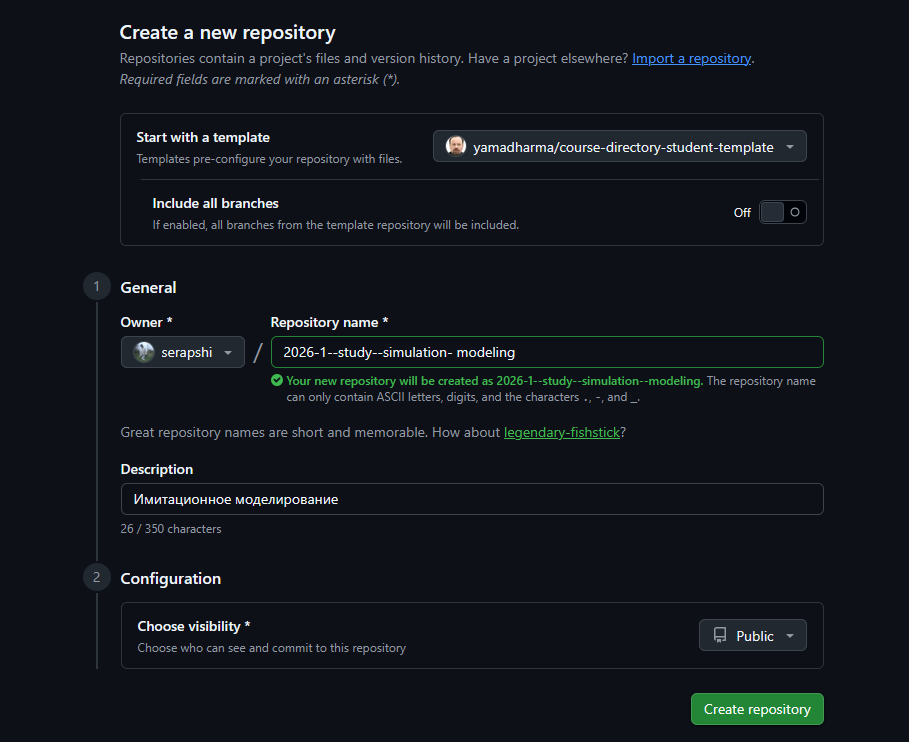
\includegraphics[width=0.7\linewidth,height=\textheight,keepaspectratio]{image/img1.png}

}

\caption{\label{fig-001}Создание репозитория}

\end{figure}%

Генерация ключа для подписи коммитов.(рис.~\ref{fig-002}).

\begin{figure}

\centering{

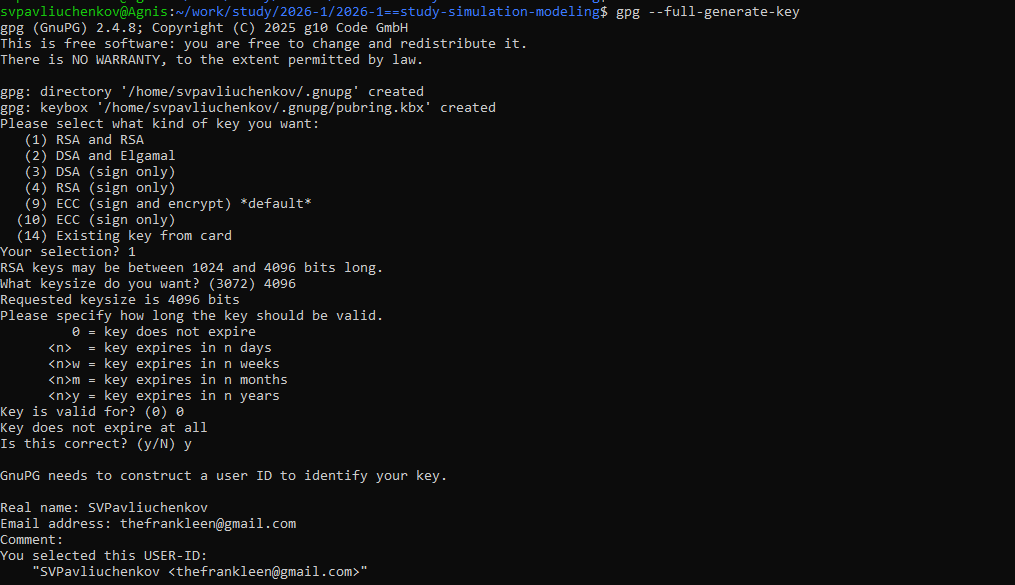
\includegraphics[width=0.7\linewidth,height=\textheight,keepaspectratio]{image/img3.png}

}

\caption{\label{fig-002}Создание gpg ключа}

\end{figure}%

Добавление скопированного ключа на гитхаб(рис.~\ref{fig-003}).

\begin{figure}

\centering{

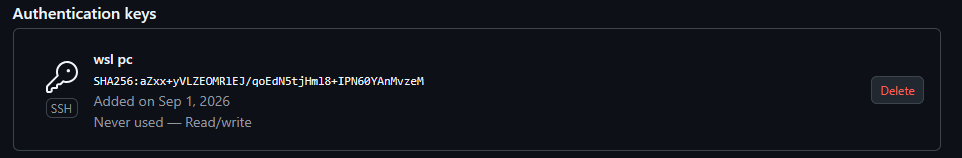
\includegraphics[width=0.7\linewidth,height=\textheight,keepaspectratio]{image/img2.png}

}

\caption{\label{fig-003}Добавление ключа на GitHub}

\end{figure}%

Установка gh(рис.~\ref{fig-004}).

\begin{figure}

\centering{

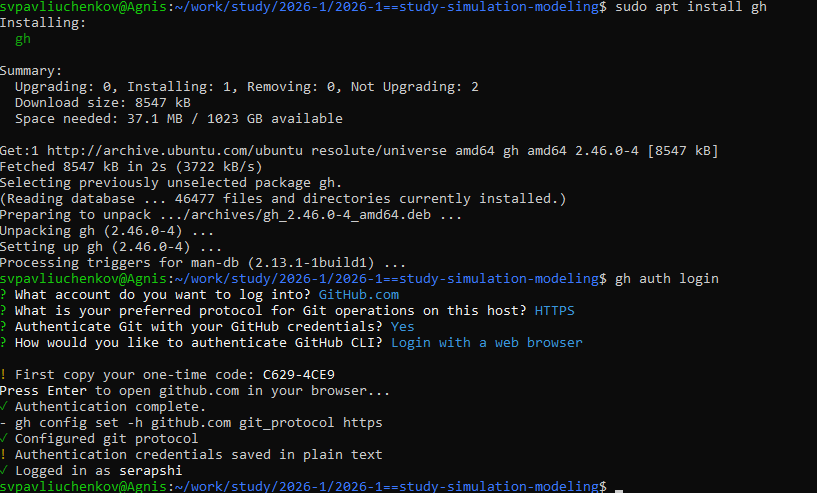
\includegraphics[width=0.7\linewidth,height=\textheight,keepaspectratio]{image/img5.png}

}

\caption{\label{fig-004}Установка необходимых пакетов}

\end{figure}%

Клонирование репозитория на виртуальную машину(рис.~\ref{fig-005}).

\begin{figure}

\centering{

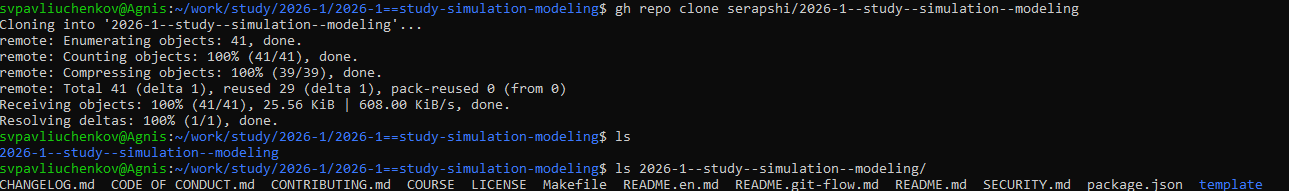
\includegraphics[width=0.7\linewidth,height=\textheight,keepaspectratio]{image/img6.png}

}

\caption{\label{fig-005}Клонирование репозитория}

\end{figure}%

Уставнока необходимых пакетов pnpm(рис.~\ref{fig-006}).

\begin{figure}

\centering{

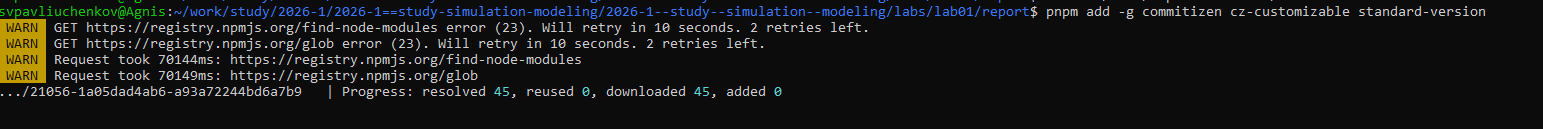
\includegraphics[width=0.7\linewidth,height=\textheight,keepaspectratio]{image/img7.png}

}

\caption{\label{fig-006}Уставнока необходимых пакетов}

\end{figure}%

Инициализация git flow(рис.~\ref{fig-007}).

\begin{figure}

\centering{

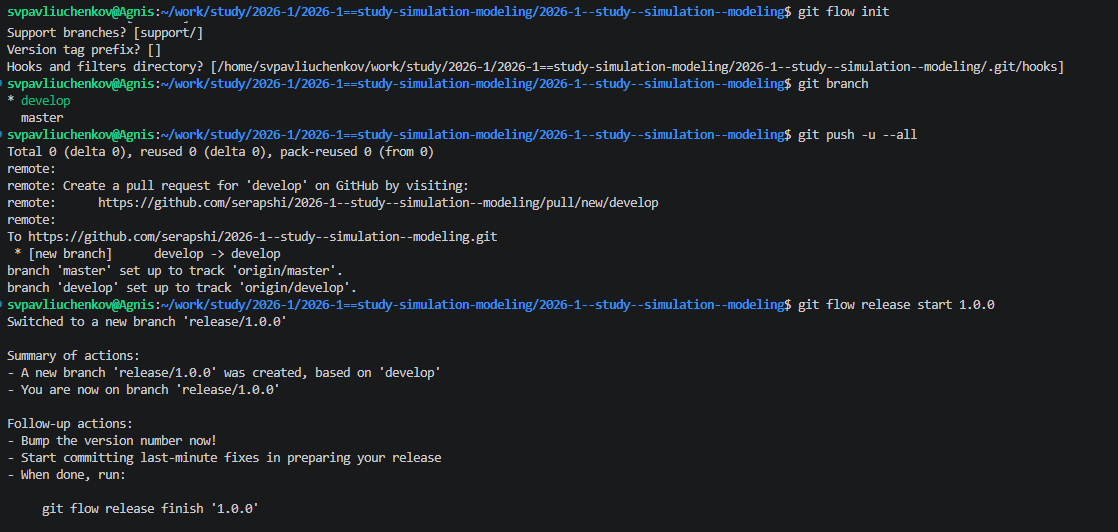
\includegraphics[width=0.7\linewidth,height=\textheight,keepaspectratio]{image/img8.png}

}

\caption{\label{fig-007}git flow}

\end{figure}%

Установка Quarto(рис.~\ref{fig-008}).

\begin{figure}

\centering{

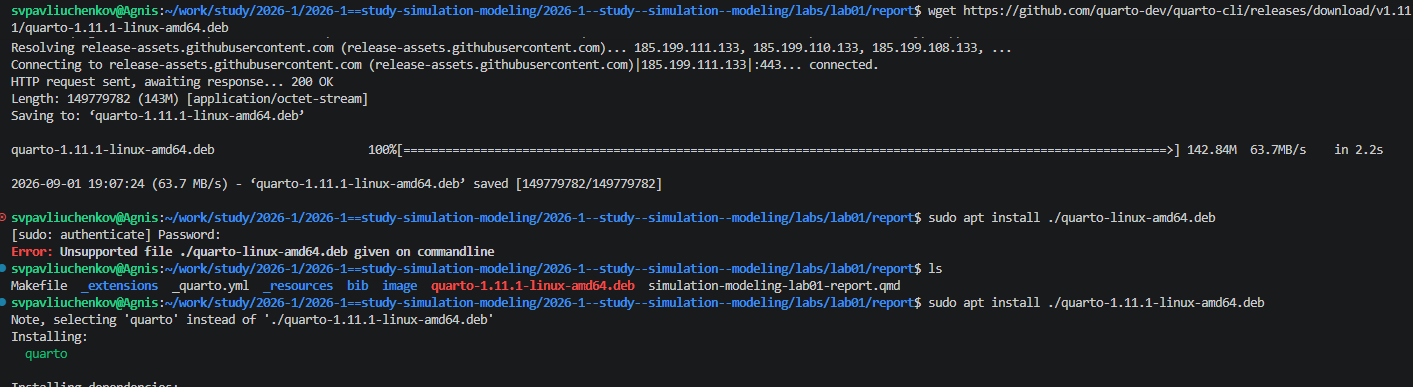
\includegraphics[width=0.7\linewidth,height=\textheight,keepaspectratio]{image/img9.png}

}

\caption{\label{fig-008}Установка Quarto}

\end{figure}%

Установка Julia(рис.~\ref{fig-009}).

\begin{figure}

\centering{

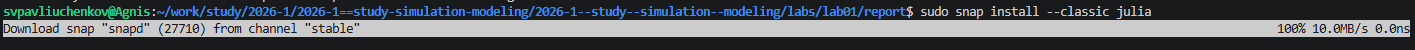
\includegraphics[width=0.7\linewidth,height=\textheight,keepaspectratio]{image/img10.png}

}

\caption{\label{fig-009}Установка Julia}

\end{figure}%

Запуск julia и добавление пакета drwatson(рис.~\ref{fig-010}).

\begin{figure}

\centering{

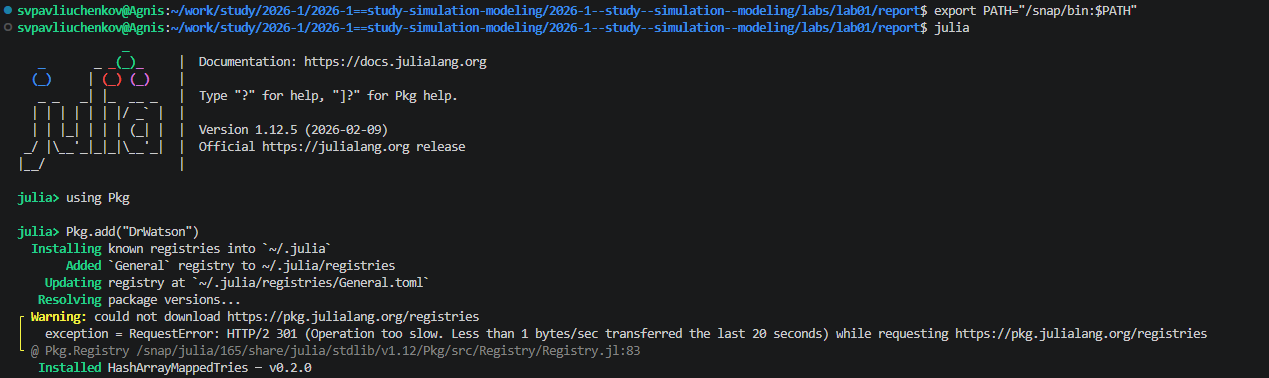
\includegraphics[width=0.7\linewidth,height=\textheight,keepaspectratio]{image/img11.png}

}

\caption{\label{fig-010}первая работа в Julia}

\end{figure}%

Добавление всех пакетов в julia с помощью add\_packages.jl и проверка
через test\_setup.jl(рис.~\ref{fig-011}).

\begin{figure}

\centering{

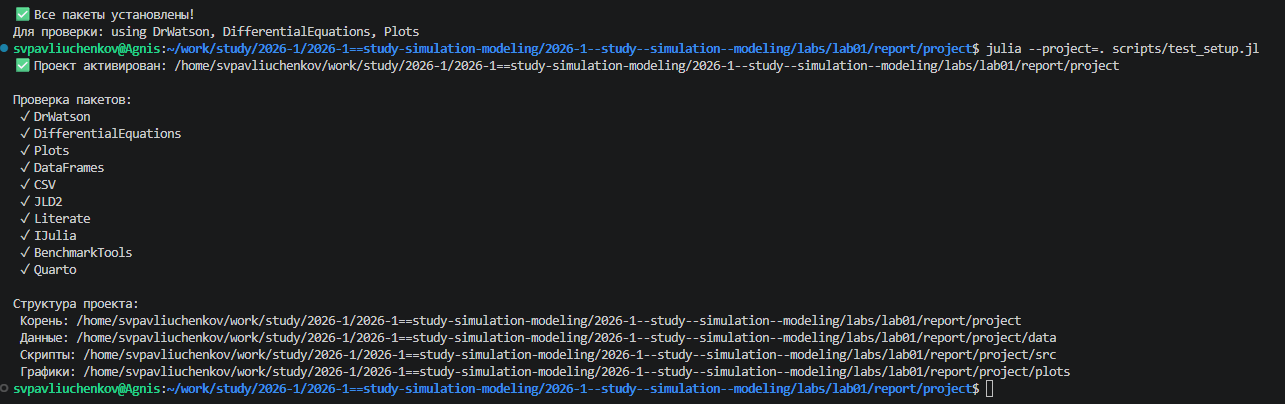
\includegraphics[width=0.7\linewidth,height=\textheight,keepaspectratio]{image/img12.png}

}

\caption{\label{fig-011}Результат test\_setup.jl}

\end{figure}%

Создаем 01\_exponential\_growth.jl. Запускаем код и получаем
результат.(рис.~\ref{fig-012}).

\begin{figure}

\centering{

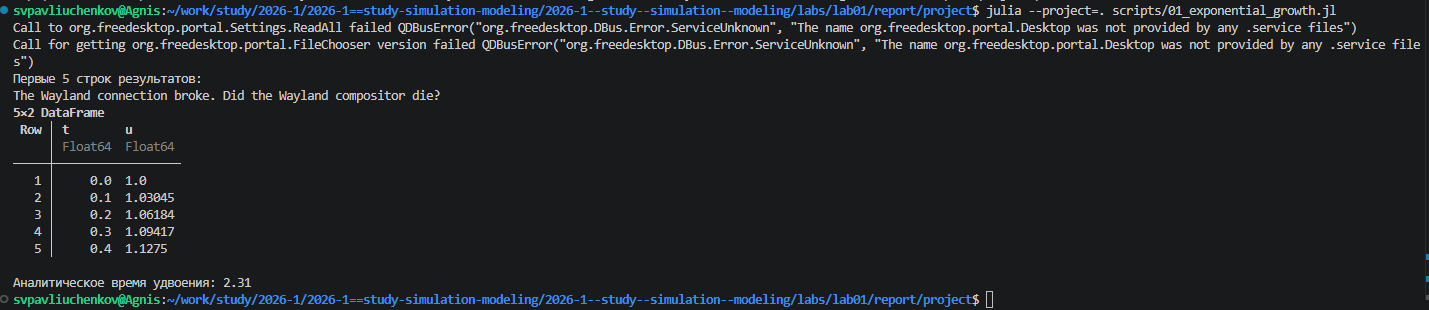
\includegraphics[width=0.7\linewidth,height=\textheight,keepaspectratio]{image/img13.png}

}

\caption{\label{fig-012}Запуск 01\_exponential\_growth.jl}

\end{figure}%

Создаем файл tangle.jl и с его помощью создаем литературные файлы для
01\_exponential\_growth.jl(рис.~\ref{fig-013}).

\begin{figure}

\centering{

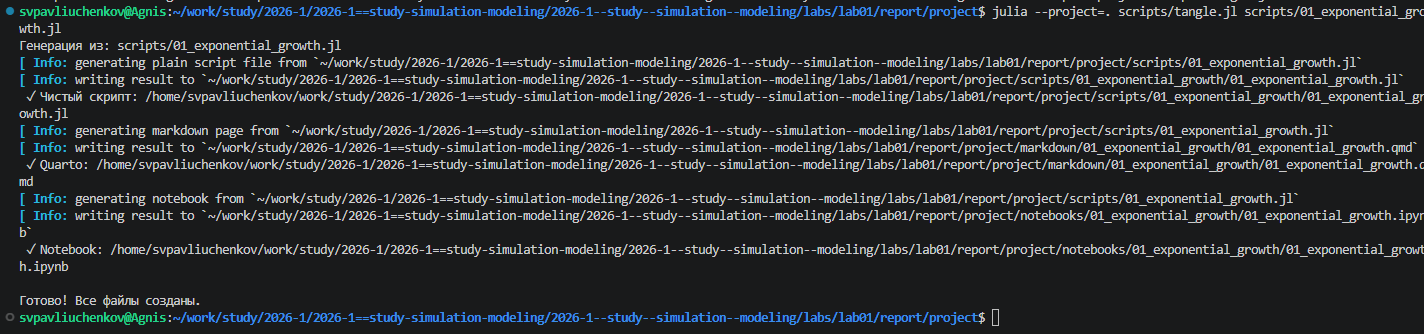
\includegraphics[width=0.7\linewidth,height=\textheight,keepaspectratio]{image/img14.png}

}

\caption{\label{fig-013}Создание литературных файлов}

\end{figure}%

\begin{Shaded}
\begin{Highlighting}[]
\ImportTok{using} \BuiltInTok{DrWatson}
\PreprocessorTok{@quickactivate} \StringTok{"project"}
\ImportTok{using} \BuiltInTok{DifferentialEquations}
\ImportTok{using} \BuiltInTok{Plots}
\ImportTok{using} \BuiltInTok{DataFrames}
\KeywordTok{function} \FunctionTok{exponential\_growth!}\NormalTok{(du, u, p, t)}
\NormalTok{α }\OperatorTok{=}\NormalTok{ p}
\NormalTok{du[}\FloatTok{1}\NormalTok{] }\OperatorTok{=}\NormalTok{ α }\OperatorTok{*}\NormalTok{ u[}\FloatTok{1}\NormalTok{]}
\KeywordTok{end}
\NormalTok{u0 }\OperatorTok{=}\NormalTok{ [}\FloatTok{1.0}\NormalTok{] }\CommentTok{\# начальная популяция}
\NormalTok{α }\OperatorTok{=} \FloatTok{0.3} \CommentTok{\# скорость роста}
\NormalTok{tspan }\OperatorTok{=}\NormalTok{ (}\FloatTok{0.0}\NormalTok{, }\FloatTok{10.0}\NormalTok{) }\CommentTok{\# временной интервал}
\NormalTok{prob }\OperatorTok{=} \FunctionTok{ODEProblem}\NormalTok{(exponential\_growth!, u0, tspan, α)}
\NormalTok{sol }\OperatorTok{=} \FunctionTok{solve}\NormalTok{(prob, }\FunctionTok{Tsit5}\NormalTok{(), saveat}\OperatorTok{=}\FloatTok{0.1}\NormalTok{)}
\FunctionTok{plot}\NormalTok{(sol, label}\OperatorTok{=}\StringTok{"u(t)"}\NormalTok{, xlabel}\OperatorTok{=}\StringTok{"Время t"}\NormalTok{, ylabel}\OperatorTok{=}\StringTok{"Популяция u"}\NormalTok{,}
\NormalTok{title}\OperatorTok{=}\StringTok{"Экспоненциальный рост (α = }\SpecialCharTok{$}\StringTok{α)", }\NormalTok{lw}\StringTok{=2, legend=:topleft)}
\FunctionTok{savefig}\NormalTok{(}\FunctionTok{plotsdir}\NormalTok{(}\StringTok{"exponential\_growth\_α=}\SpecialCharTok{$}\StringTok{α.}\NormalTok{png}\StringTok{"}\NormalTok{))}
\NormalTok{df }\OperatorTok{=} \FunctionTok{DataFrame}\NormalTok{(t}\OperatorTok{=}\NormalTok{sol.t, u}\OperatorTok{=}\FunctionTok{first}\NormalTok{.(sol.u))}
\FunctionTok{println}\NormalTok{(}\StringTok{"Первые 5 строк результатов:"}\NormalTok{)}
\FunctionTok{println}\NormalTok{(}\FunctionTok{first}\NormalTok{(df, }\FloatTok{5}\NormalTok{))}
\NormalTok{u\_final }\OperatorTok{=} \FunctionTok{last}\NormalTok{(sol.u)[}\FloatTok{1}\NormalTok{]}
\NormalTok{doubling\_time }\OperatorTok{=} \FunctionTok{log}\NormalTok{(}\FloatTok{2}\NormalTok{) }\OperatorTok{/}\NormalTok{ α}
\FunctionTok{println}\NormalTok{(}\StringTok{"}\SpecialCharTok{\textbackslash{}n}\StringTok{Аналитическое время удвоения: "}\NormalTok{, }\FunctionTok{round}\NormalTok{(doubling\_time;digits}\OperatorTok{=}\FloatTok{2}\NormalTok{))}
\end{Highlighting}
\end{Shaded}

\begin{verbatim}
Первые 5 строк результатов:
5×2 DataFrame
 Row │ t        u       
     │ Float64  Float64 
─────┼──────────────────
   1 │     0.0  1.0
   2 │     0.1  1.03045
   3 │     0.2  1.06184
   4 │     0.3  1.09417
   5 │     0.4  1.1275

Аналитическое время удвоения: 2.31
\end{verbatim}

Создаем 01\_exponential\_growth.jl, проделоваем аналогичные действия и
получаем.

\chapter{Параметрическое исследование экспоненциального
роста}\label{ux43fux430ux440ux430ux43cux435ux442ux440ux438ux447ux435ux441ux43aux43eux435-ux438ux441ux441ux43bux435ux434ux43eux432ux430ux43dux438ux435-ux44dux43aux441ux43fux43eux43dux435ux43dux446ux438ux430ux43bux44cux43dux43eux433ux43e-ux440ux43eux441ux442ux430}

\section{Активация проекта и загрузка
пакетов}\label{ux430ux43aux442ux438ux432ux430ux446ux438ux44f-ux43fux440ux43eux435ux43aux442ux430-ux438-ux437ux430ux433ux440ux443ux437ux43aux430-ux43fux430ux43aux435ux442ux43eux432}

\textbf{ИЗМЕНЕНИЕ:} Добавлен DrWatson для управления проектом и
параметрами

\begin{Shaded}
\begin{Highlighting}[]
\ImportTok{using} \BuiltInTok{DrWatson}
\PreprocessorTok{@quickactivate} \StringTok{"project"} \CommentTok{\# Активация проекта DrWatson}
\ImportTok{using} \BuiltInTok{DifferentialEquations}
\ImportTok{using} \BuiltInTok{DataFrames}
\ImportTok{using} \BuiltInTok{Plots}
\ImportTok{using} \BuiltInTok{JLD2}
\ImportTok{using} \BuiltInTok{BenchmarkTools}
\end{Highlighting}
\end{Shaded}

Установка каталогов

\begin{Shaded}
\begin{Highlighting}[]
\NormalTok{script\_name }\OperatorTok{=} \FunctionTok{splitext}\NormalTok{(}\FunctionTok{basename}\NormalTok{(}\ConstantTok{PROGRAM\_FILE}\NormalTok{))[}\FloatTok{1}\NormalTok{]}
\FunctionTok{mkpath}\NormalTok{(}\FunctionTok{plotsdir}\NormalTok{(script\_name))}
\FunctionTok{mkpath}\NormalTok{(}\FunctionTok{datadir}\NormalTok{(script\_name))}
\end{Highlighting}
\end{Shaded}

\begin{verbatim}
"/home/svpavliuchenkov/work/study/2026-1/2026-1==study-simulation-modeling/2026-1--study--simulation--modeling/labs/lab01/project/data/startup"
\end{verbatim}

\section{Определение
модели}\label{ux43eux43fux440ux435ux434ux435ux43bux435ux43dux438ux435-ux43cux43eux434ux435ux43bux438}

Модель: 𝑑𝑢/𝑑𝑡 = 𝛼 ⋅ 𝑢

\begin{Shaded}
\begin{Highlighting}[]
\KeywordTok{function} \FunctionTok{exponential\_growth!}\NormalTok{(du, u, p, t)}
\NormalTok{α }\OperatorTok{=}\NormalTok{ p.α }\CommentTok{\# **ИЗМЕНЕНИЕ:** Параметры теперь передаются как именованный кортеж↪}
\NormalTok{du[}\FloatTok{1}\NormalTok{] }\OperatorTok{=}\NormalTok{ α }\OperatorTok{*}\NormalTok{ u[}\FloatTok{1}\NormalTok{]}
\KeywordTok{end}
\end{Highlighting}
\end{Shaded}

\begin{verbatim}
exponential_growth! (generic function with 1 method)
\end{verbatim}

\section{Определение параметров в
Dict}\label{ux43eux43fux440ux435ux434ux435ux43bux435ux43dux438ux435-ux43fux430ux440ux430ux43cux435ux442ux440ux43eux432-ux432-dict}

\textbf{ОСНОВНОЕ ИЗМЕНЕНИЕ:} Все параметры собраны в Dict для
систематизации↪ Базовый набор параметров (один эксперимент)

\begin{Shaded}
\begin{Highlighting}[]
\NormalTok{base\_params }\OperatorTok{=} \FunctionTok{Dict}\NormalTok{(}
\OperatorTok{:}\NormalTok{u0 }\OperatorTok{=\textgreater{}}\NormalTok{ [}\FloatTok{1.0}\NormalTok{], }\CommentTok{\# начальная популяция}
\OperatorTok{:}\NormalTok{α }\OperatorTok{=\textgreater{}} \FloatTok{0.3}\NormalTok{, }\CommentTok{\# скорость роста}
\OperatorTok{:}\NormalTok{tspan }\OperatorTok{=\textgreater{}}\NormalTok{ (}\FloatTok{0.0}\NormalTok{, }\FloatTok{10.0}\NormalTok{), }\CommentTok{\# интервал времени}
\OperatorTok{:}\NormalTok{solver }\OperatorTok{=\textgreater{}} \FunctionTok{Tsit5}\NormalTok{(), }\CommentTok{\# метод решения}
\OperatorTok{:}\NormalTok{saveat }\OperatorTok{=\textgreater{}} \FloatTok{0.1}\NormalTok{, }\CommentTok{\# шаг сохранения результатов}
\OperatorTok{:}\NormalTok{experiment\_name }\OperatorTok{=\textgreater{}} \StringTok{"base\_experiment"}
\NormalTok{)}
\FunctionTok{println}\NormalTok{(}\StringTok{"Базовые параметры эксперимента:"}\NormalTok{)}
\ControlFlowTok{for}\NormalTok{ (key, value) }\KeywordTok{in}\NormalTok{ base\_params}
\FunctionTok{println}\NormalTok{(}\StringTok{" }\SpecialCharTok{$}\NormalTok{key}\StringTok{ = }\SpecialCharTok{$}\NormalTok{value}\StringTok{"}\NormalTok{)}
\ControlFlowTok{end}
\end{Highlighting}
\end{Shaded}

\begin{verbatim}
Базовые параметры эксперимента:
 α = 0.3
 u0 = [1.0]
 saveat = 0.1
 solver = OrdinaryDiffEqTsit5.Tsit5{typeof(OrdinaryDiffEqCore.trivial_limiter!), typeof(OrdinaryDiffEqCore.trivial_limiter!), FastBroadcast.Serial}(OrdinaryDiffEqCore.trivial_limiter!, OrdinaryDiffEqCore.trivial_limiter!, FastBroadcast.Serial())
 experiment_name = base_experiment
 tspan = (0.0, 10.0)
\end{verbatim}

\section{Функция-обертка для запуска одного
эксперимента}\label{ux444ux443ux43dux43aux446ux438ux44f-ux43eux431ux435ux440ux442ux43aux430-ux434ux43bux44f-ux437ux430ux43fux443ux441ux43aux430-ux43eux434ux43dux43eux433ux43e-ux44dux43aux441ux43fux435ux440ux438ux43cux435ux43dux442ux430}

\textbf{ИСПРАВЛЕНИЕ:} Возвращаем Dict со строковыми ключами

\begin{Shaded}
\begin{Highlighting}[]
\KeywordTok{function} \FunctionTok{run\_single\_experiment}\NormalTok{(params}\OperatorTok{::}\DataTypeTok{Dict}\NormalTok{)}
\PreprocessorTok{@unpack}\NormalTok{ u0, α, tspan, solver, saveat }\OperatorTok{=}\NormalTok{ params}
\NormalTok{prob }\OperatorTok{=} \FunctionTok{ODEProblem}\NormalTok{(exponential\_growth!, u0, tspan, (α}\OperatorTok{=}\NormalTok{α,)) }\CommentTok{\# Создаем и решаем задачу↪}
\NormalTok{sol }\OperatorTok{=} \FunctionTok{solve}\NormalTok{(prob, solver; saveat}\OperatorTok{=}\NormalTok{saveat)}
\NormalTok{final\_population }\OperatorTok{=} \FunctionTok{last}\NormalTok{(sol.u)[}\FloatTok{1}\NormalTok{] }\CommentTok{\# Анализ результатов}
\NormalTok{doubling\_time }\OperatorTok{=} \FunctionTok{log}\NormalTok{(}\FloatTok{2}\NormalTok{) }\OperatorTok{/}\NormalTok{ α}
\ControlFlowTok{return} \FunctionTok{Dict}\NormalTok{(}
\StringTok{"solution"} \OperatorTok{=\textgreater{}}\NormalTok{ sol,}
\StringTok{"time\_points"} \OperatorTok{=\textgreater{}}\NormalTok{ sol.t,}
\StringTok{"population\_values"} \OperatorTok{=\textgreater{}} \FunctionTok{first}\NormalTok{.(sol.u),}
\StringTok{"final\_population"} \OperatorTok{=\textgreater{}}\NormalTok{ final\_population,}
\StringTok{"doubling\_time"} \OperatorTok{=\textgreater{}}\NormalTok{ doubling\_time,}
\StringTok{"parameters"} \OperatorTok{=\textgreater{}}\NormalTok{ params }\CommentTok{\# Сохраняем исходные параметры}
\NormalTok{) }\CommentTok{\# Используем строки как ключи для совместимости с DrWatson}
\KeywordTok{end}
\end{Highlighting}
\end{Shaded}

\begin{verbatim}
run_single_experiment (generic function with 1 method)
\end{verbatim}

\section{Запуск базового
эксперимента}\label{ux437ux430ux43fux443ux441ux43a-ux431ux430ux437ux43eux432ux43eux433ux43e-ux44dux43aux441ux43fux435ux440ux438ux43cux435ux43dux442ux430}

\textbf{ИЗМЕНЕНИЕ:} Используем produce\_or\_load для автоматического
кэширования↪

\begin{Shaded}
\begin{Highlighting}[]
\NormalTok{data, path }\OperatorTok{=} \FunctionTok{produce\_or\_load}\NormalTok{(}
\FunctionTok{datadir}\NormalTok{(script\_name, }\StringTok{"single"}\NormalTok{), }\CommentTok{\# Папка для сохранения}
\NormalTok{base\_params, }\CommentTok{\# Параметры эксперимента}
\NormalTok{run\_single\_experiment, }\CommentTok{\# Функция для выполнения}
\NormalTok{prefix }\OperatorTok{=} \StringTok{"exp\_growth"}\NormalTok{, }\CommentTok{\# Префикс имени файла}
\NormalTok{tag }\OperatorTok{=} \ConstantTok{false}\NormalTok{, }\CommentTok{\# Не добавлять git{-}тег}
\NormalTok{verbose }\OperatorTok{=} \ConstantTok{true}
\NormalTok{)}
\FunctionTok{println}\NormalTok{(}\StringTok{"}\SpecialCharTok{\textbackslash{}n}\StringTok{Результаты базового эксперимента:"}\NormalTok{)}
\FunctionTok{println}\NormalTok{(}\StringTok{" Финальная популяция: "}\NormalTok{, data[}\StringTok{"final\_population"}\NormalTok{])}
\FunctionTok{println}\NormalTok{(}\StringTok{" Время удвоения: "}\NormalTok{, }\FunctionTok{round}\NormalTok{(data[}\StringTok{"doubling\_time"}\NormalTok{]; digits}\OperatorTok{=}\FloatTok{2}\NormalTok{))}
\FunctionTok{println}\NormalTok{(}\StringTok{" Файл результатов: "}\NormalTok{, path)}
\end{Highlighting}
\end{Shaded}

\begin{verbatim}

Результаты базового эксперимента:
 Финальная популяция: 20.08544851618676
 Время удвоения: 2.31
 Файл результатов: /home/svpavliuchenkov/work/study/2026-1/2026-1==study-simulation-modeling/2026-1--study--simulation--modeling/labs/lab01/project/data/startup/single/exp_growth_experiment_name=base_experiment_saveat=0.1_α=0.3.jld2
\end{verbatim}

\section{Визуализация базового
эксперимента}\label{ux432ux438ux437ux443ux430ux43bux438ux437ux430ux446ux438ux44f-ux431ux430ux437ux43eux432ux43eux433ux43e-ux44dux43aux441ux43fux435ux440ux438ux43cux435ux43dux442ux430}

\begin{Shaded}
\begin{Highlighting}[]
\NormalTok{p1 }\OperatorTok{=} \FunctionTok{plot}\NormalTok{(data[}\StringTok{"time\_points"}\NormalTok{], data[}\StringTok{"population\_values"}\NormalTok{],}
\NormalTok{label}\OperatorTok{=}\StringTok{"α = }\SpecialCharTok{$}\NormalTok{(base\_params[}\OperatorTok{:}\NormalTok{α])}\StringTok{"}\NormalTok{,}
\NormalTok{xlabel}\OperatorTok{=}\StringTok{"Время, t"}\NormalTok{,}
\NormalTok{ylabel}\OperatorTok{=}\StringTok{"Популяция, u(t)"}\NormalTok{,}
\NormalTok{title}\OperatorTok{=}\StringTok{"Экспоненциальный рост (базовый эксперимент)"}\NormalTok{,}
\NormalTok{lw}\OperatorTok{=}\FloatTok{2}\NormalTok{,}
\NormalTok{legend}\OperatorTok{=:}\NormalTok{topleft,grid}\OperatorTok{=}\ConstantTok{true}
\NormalTok{)}
\end{Highlighting}
\end{Shaded}

\pandocbounded{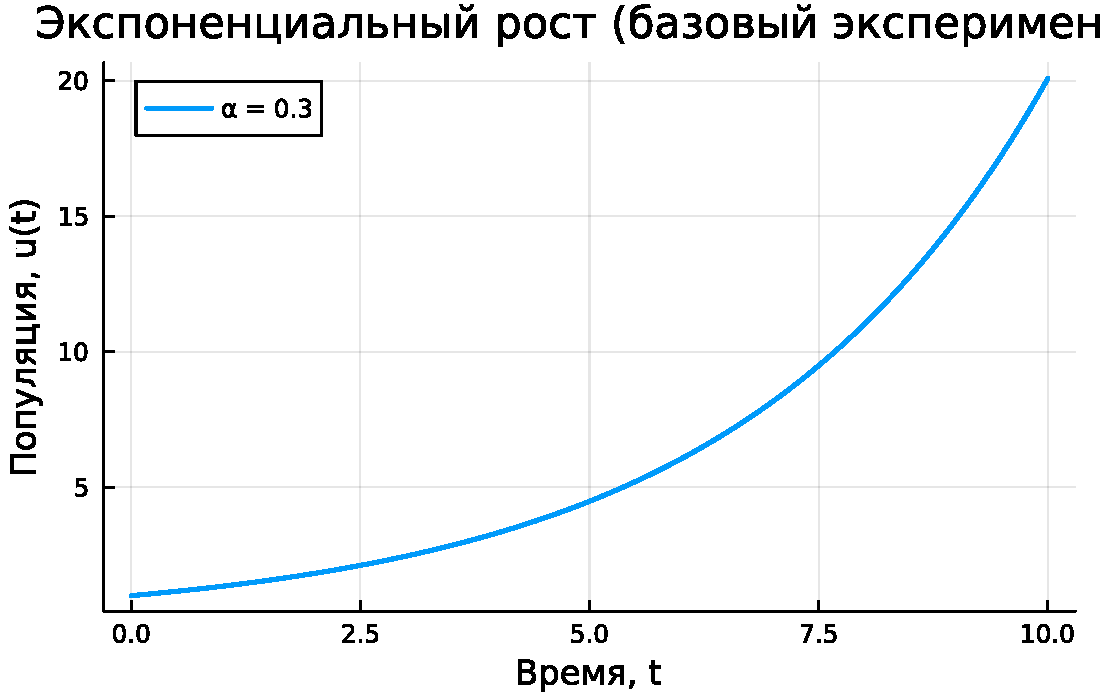
\includegraphics[keepaspectratio]{simulation-modeling-lab01-report_files/figure-pdf/cell-9-output-1.pdf}}

Сохраним график в папку plots

\begin{Shaded}
\begin{Highlighting}[]
\FunctionTok{savefig}\NormalTok{(}\FunctionTok{plotsdir}\NormalTok{(script\_name, }\StringTok{"single\_experiment.png"}\NormalTok{))}
\end{Highlighting}
\end{Shaded}

\begin{verbatim}
"/home/svpavliuchenkov/work/study/2026-1/2026-1==study-simulation-modeling/2026-1--study--simulation--modeling/labs/lab01/project/plots/startup/single_experiment.png"
\end{verbatim}

\section{Параметрическое
сканирование}\label{ux43fux430ux440ux430ux43cux435ux442ux440ux438ux447ux435ux441ux43aux43eux435-ux441ux43aux430ux43dux438ux440ux43eux432ux430ux43dux438ux435}

\textbf{НОВАЯ СЕКЦИЯ:} Исследование влияния параметра α Сетка параметров
для сканирования

\begin{Shaded}
\begin{Highlighting}[]
\NormalTok{param\_grid }\OperatorTok{=} \FunctionTok{Dict}\NormalTok{(}
\OperatorTok{:}\NormalTok{u0 }\OperatorTok{=\textgreater{}}\NormalTok{ [[}\FloatTok{1.0}\NormalTok{]], }\CommentTok{\# фиксируем начальное условие}
\OperatorTok{:}\NormalTok{α }\OperatorTok{=\textgreater{}}\NormalTok{ [}\FloatTok{0.1}\NormalTok{, }\FloatTok{0.3}\NormalTok{, }\FloatTok{0.5}\NormalTok{, }\FloatTok{0.8}\NormalTok{, }\FloatTok{1.0}\NormalTok{], }\CommentTok{\# исследуемые значения скоростироста↪}
\OperatorTok{:}\NormalTok{tspan }\OperatorTok{=\textgreater{}}\NormalTok{ [(}\FloatTok{0.0}\NormalTok{, }\FloatTok{10.0}\NormalTok{)], }\CommentTok{\# фиксируем интервал времени}
\OperatorTok{:}\NormalTok{solver }\OperatorTok{=\textgreater{}}\NormalTok{ [}\FunctionTok{Tsit5}\NormalTok{()], }\CommentTok{\# фиксируем метод решения}
\OperatorTok{:}\NormalTok{saveat }\OperatorTok{=\textgreater{}}\NormalTok{ [}\FloatTok{0.1}\NormalTok{], }\CommentTok{\# фиксируем шаг сохранения}
\OperatorTok{:}\NormalTok{experiment\_name }\OperatorTok{=\textgreater{}}\NormalTok{ [}\StringTok{"parametric\_scan"}\NormalTok{]}
\NormalTok{)}
\end{Highlighting}
\end{Shaded}

\begin{verbatim}
Dict{Symbol, Vector} with 6 entries:
  :α               => [0.1, 0.3, 0.5, 0.8, 1.0]
  :u0              => [[1.0]]
  :saveat          => [0.1]
  :solver          => [Tsit5{typeof(trivial_limiter!), typeof(trivial_limiter!)…
  :experiment_name => ["parametric_scan"]
  :tspan           => [(0.0, 10.0)]
\end{verbatim}

Генерация всех комбинаций параметров

\begin{Shaded}
\begin{Highlighting}[]
\NormalTok{all\_params }\OperatorTok{=} \FunctionTok{dict\_list}\NormalTok{(param\_grid)}
\FunctionTok{println}\NormalTok{(}\StringTok{"}\SpecialCharTok{\textbackslash{}n}\StringTok{"} \OperatorTok{*} \StringTok{"="}\OperatorTok{\^{}}\FloatTok{60}\NormalTok{)}
\FunctionTok{println}\NormalTok{(}\StringTok{"ПАРАМЕТРИЧЕСКОЕ СКАНИРОВАНИЕ"}\NormalTok{)}
\FunctionTok{println}\NormalTok{(}\StringTok{"Всего комбинаций параметров: "}\NormalTok{, }\FunctionTok{length}\NormalTok{(all\_params))}
\FunctionTok{println}\NormalTok{(}\StringTok{"Исследуемые значения α: "}\NormalTok{, param\_grid[}\OperatorTok{:}\NormalTok{α])}
\FunctionTok{println}\NormalTok{(}\StringTok{"="}\OperatorTok{\^{}}\FloatTok{60}\NormalTok{)}
\end{Highlighting}
\end{Shaded}

\begin{verbatim}

============================================================
ПАРАМЕТРИЧЕСКОЕ СКАНИРОВАНИЕ
Всего комбинаций параметров: 5
Исследуемые значения α: [0.1, 0.3, 0.5, 0.8, 1.0]
============================================================
\end{verbatim}

\section{Запуск всех экспериментов и собор
результатов}\label{ux437ux430ux43fux443ux441ux43a-ux432ux441ux435ux445-ux44dux43aux441ux43fux435ux440ux438ux43cux435ux43dux442ux43eux432-ux438-ux441ux43eux431ux43eux440-ux440ux435ux437ux443ux43bux44cux442ux430ux442ux43eux432}

\textbf{НОВАЯ СЕКЦИЯ:} Автоматический запуск и сохранение всех вариантов

\begin{Shaded}
\begin{Highlighting}[]
\NormalTok{all\_results }\OperatorTok{=}\NormalTok{ []}
\NormalTok{all\_dfs }\OperatorTok{=}\NormalTok{ []}
\ControlFlowTok{for}\NormalTok{ (i, params) }\KeywordTok{in} \FunctionTok{enumerate}\NormalTok{(all\_params)}
\FunctionTok{println}\NormalTok{(}\StringTok{"Прогресс: }\SpecialCharTok{$}\NormalTok{i}\StringTok{/}\SpecialCharTok{$}\NormalTok{(}\FunctionTok{length}\NormalTok{(all\_params))}\StringTok{ | α = }\SpecialCharTok{$}\NormalTok{(params[}\OperatorTok{:}\NormalTok{α])}\StringTok{"}\NormalTok{)}
\NormalTok{data, path }\OperatorTok{=} \FunctionTok{produce\_or\_load}\NormalTok{(}
\FunctionTok{datadir}\NormalTok{(script\_name, }\StringTok{"parametric\_scan"}\NormalTok{), }\CommentTok{\# Данные}
\NormalTok{params, }\CommentTok{\# Текущий набор параметров}
\NormalTok{run\_single\_experiment, }\CommentTok{\# Функция для выполнения}
\NormalTok{prefix }\OperatorTok{=} \StringTok{"scan"}\NormalTok{, }\CommentTok{\# Префикс имени файла}
\NormalTok{tag }\OperatorTok{=} \ConstantTok{false}\NormalTok{,verbose }\OperatorTok{=} \ConstantTok{false} \CommentTok{\# Не выводить подробности длякаждого запуска↪}
\NormalTok{) }\CommentTok{\# Автоматическое сохранение/загрузка каждого эксперимента}
\NormalTok{result\_summary }\OperatorTok{=} \FunctionTok{merge}\NormalTok{(}
\NormalTok{params,}
\FunctionTok{Dict}\NormalTok{(}
\OperatorTok{:}\NormalTok{final\_population }\OperatorTok{=\textgreater{}}\NormalTok{ data[}\StringTok{"final\_population"}\NormalTok{],}
\OperatorTok{:}\NormalTok{doubling\_time }\OperatorTok{=\textgreater{}}\NormalTok{ data[}\StringTok{"doubling\_time"}\NormalTok{],}
\OperatorTok{:}\NormalTok{filepath }\OperatorTok{=\textgreater{}}\NormalTok{ path }\CommentTok{\# Путь к сохраненным данным}
\NormalTok{)}
\NormalTok{) }\CommentTok{\# Сохраняем сводные результаты (используем символы дляпараметров, но данные из data {-} строки}

\FunctionTok{push!}\NormalTok{(all\_results, result\_summary)}
\NormalTok{df }\OperatorTok{=} \FunctionTok{DataFrame}\NormalTok{(}
\NormalTok{t }\OperatorTok{=}\NormalTok{ data[}\StringTok{"time\_points"}\NormalTok{],}
\NormalTok{u }\OperatorTok{=}\NormalTok{ data[}\StringTok{"population\_values"}\NormalTok{],}
\NormalTok{α }\OperatorTok{=} \FunctionTok{fill}\NormalTok{(params[}\OperatorTok{:}\NormalTok{α], }\FunctionTok{length}\NormalTok{(data[}\StringTok{"time\_points"}\NormalTok{]))}
\NormalTok{) }\CommentTok{\# Сохраняем полные данные для визуализации}
\FunctionTok{push!}\NormalTok{(all\_dfs, df)}
\ControlFlowTok{end}
\end{Highlighting}
\end{Shaded}

\begin{verbatim}
Прогресс: 1/5 | α = 0.1
Прогресс: 2/5 | α = 0.3
Прогресс: 3/5 | α = 0.5
Прогресс: 4/5 | α = 0.8
Прогресс: 5/5 | α = 1.0
\end{verbatim}

\section{Анализ и визуализация результатов
сканирования}\label{ux430ux43dux430ux43bux438ux437-ux438-ux432ux438ux437ux443ux430ux43bux438ux437ux430ux446ux438ux44f-ux440ux435ux437ux443ux43bux44cux442ux430ux442ux43eux432-ux441ux43aux430ux43dux438ux440ux43eux432ux430ux43dux438ux44f}

\textbf{НОВАЯ СЕКЦИЯ:} Сравнительный анализ всех экспериментов Сводная
таблица результатов

\begin{Shaded}
\begin{Highlighting}[]
\NormalTok{results\_df }\OperatorTok{=} \FunctionTok{DataFrame}\NormalTok{(all\_results)}
\FunctionTok{println}\NormalTok{(}\StringTok{"}\SpecialCharTok{\textbackslash{}n}\StringTok{Сводная таблица результатов:"}\NormalTok{)}
\FunctionTok{println}\NormalTok{(results\_df[!, [}\OperatorTok{:}\NormalTok{α, }\OperatorTok{:}\NormalTok{final\_population, }\OperatorTok{:}\NormalTok{doubling\_time]])}
\end{Highlighting}
\end{Shaded}

\begin{verbatim}

Сводная таблица результатов:
5×3 DataFrame
 Row │ α        final_population  doubling_time 
     │ Float64  Float64           Float64       
─────┼──────────────────────────────────────────
   1 │     0.1           2.71828       6.93147
   2 │     0.3          20.0854        2.31049
   3 │     0.5         148.409         1.38629
   4 │     0.8        2980.57          0.866434
   5 │     1.0       22021.0           0.693147
\end{verbatim}

Сравнительный график всех траекторий

\begin{Shaded}
\begin{Highlighting}[]
\NormalTok{p2 }\OperatorTok{=} \FunctionTok{plot}\NormalTok{(size}\OperatorTok{=}\NormalTok{(}\FloatTok{800}\NormalTok{, }\FloatTok{500}\NormalTok{), dpi}\OperatorTok{=}\FloatTok{150}\NormalTok{)}
\ControlFlowTok{for}\NormalTok{ params }\KeywordTok{in}\NormalTok{ all\_params}
\NormalTok{data, \_ }\OperatorTok{=} \FunctionTok{produce\_or\_load}\NormalTok{(}
\FunctionTok{datadir}\NormalTok{(script\_name, }\StringTok{"parametric\_scan"}\NormalTok{),}
\NormalTok{params,}
\NormalTok{run\_single\_experiment,}
\NormalTok{prefix }\OperatorTok{=} \StringTok{"scan"}
\NormalTok{) }\CommentTok{\# Загружаем данные (они уже есть на диске)}
\FunctionTok{plot!}\NormalTok{(p2, data[}\StringTok{"time\_points"}\NormalTok{], data[}\StringTok{"population\_values"}\NormalTok{],}
\NormalTok{label}\OperatorTok{=}\StringTok{"α = }\SpecialCharTok{$}\NormalTok{(params[}\OperatorTok{:}\NormalTok{α])}\StringTok{"}\NormalTok{,}
\NormalTok{lw}\OperatorTok{=}\FloatTok{2}\NormalTok{,}
\NormalTok{alpha}\OperatorTok{=}\FloatTok{0.8}
\NormalTok{)}
\ControlFlowTok{end}
\FunctionTok{plot!}\NormalTok{(p2,}
\NormalTok{xlabel}\OperatorTok{=}\StringTok{"Время, t"}\NormalTok{,}
\NormalTok{ylabel}\OperatorTok{=}\StringTok{"Популяция, u(t)"}\NormalTok{,}
\NormalTok{title}\OperatorTok{=}\StringTok{"Параметрическое исследование: влияние α на рост"}\NormalTok{,}
\NormalTok{legend}\OperatorTok{=:}\NormalTok{topleft,}
\NormalTok{grid}\OperatorTok{=}\ConstantTok{true}
\NormalTok{)}
\end{Highlighting}
\end{Shaded}

\pandocbounded{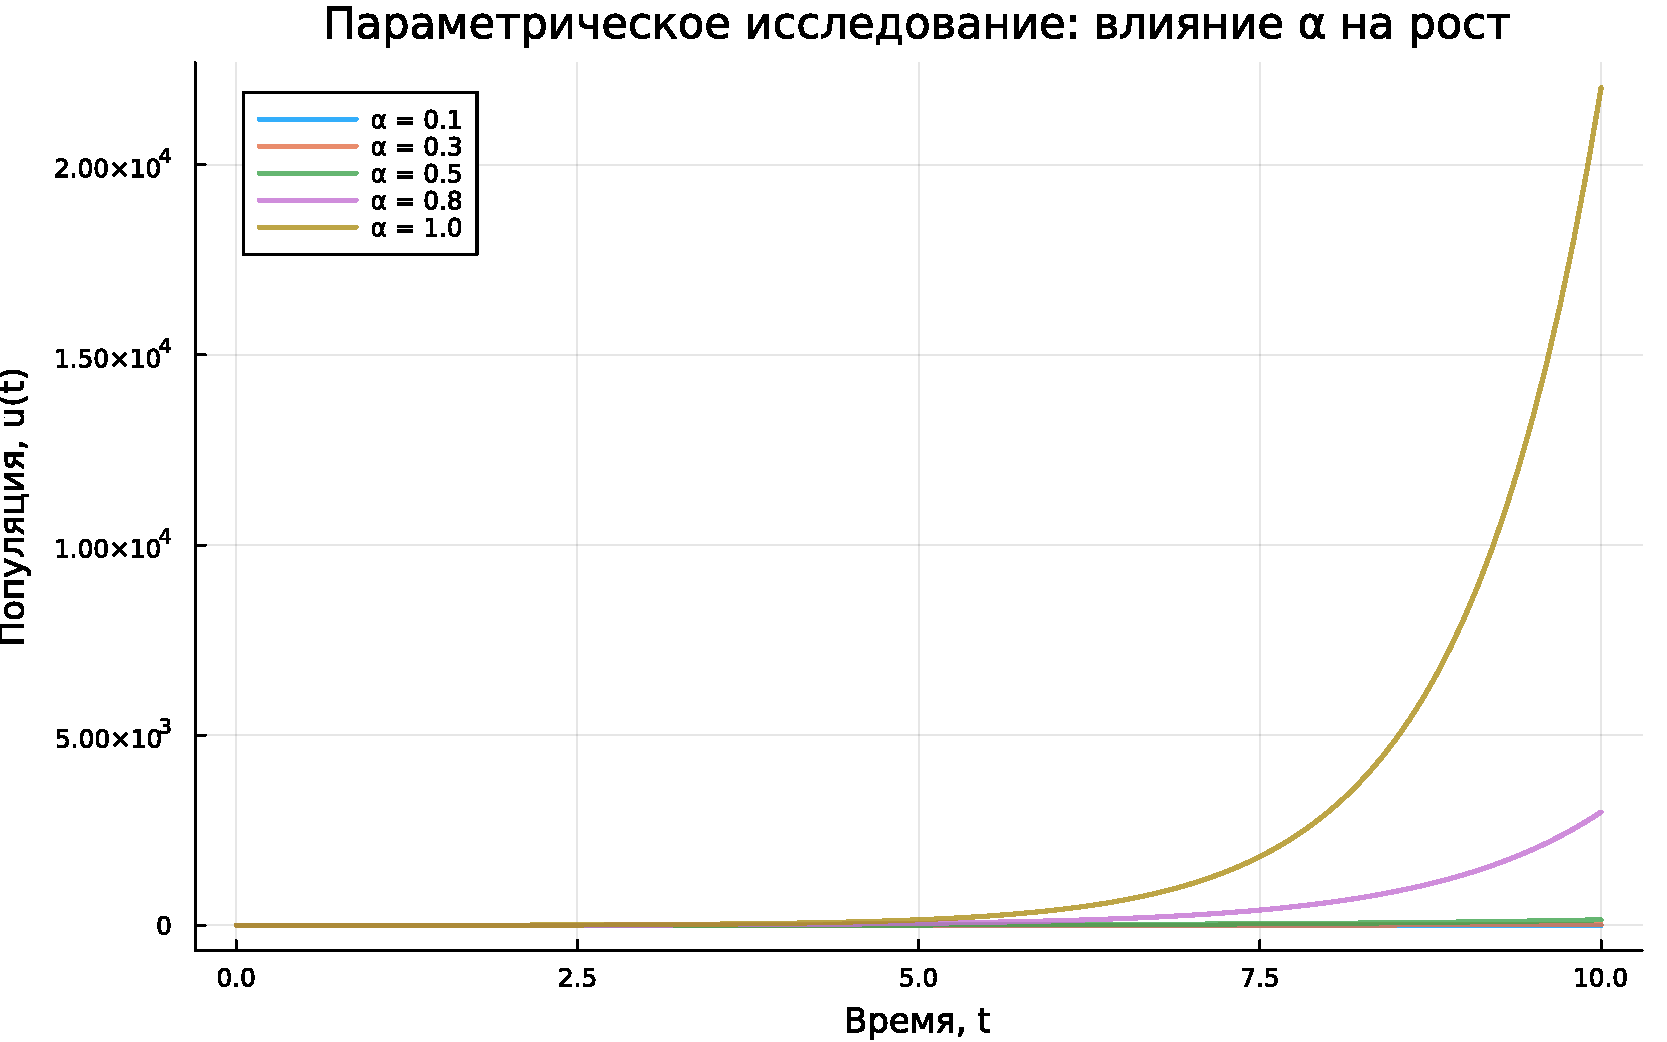
\includegraphics[keepaspectratio]{simulation-modeling-lab01-report_files/figure-pdf/cell-15-output-1.pdf}}

Сохраним график в папку plots

\begin{Shaded}
\begin{Highlighting}[]
\FunctionTok{savefig}\NormalTok{(}\FunctionTok{plotsdir}\NormalTok{(script\_name, }\StringTok{"parametric\_scan\_comparison.png"}\NormalTok{))}
\end{Highlighting}
\end{Shaded}

\begin{verbatim}
"/home/svpavliuchenkov/work/study/2026-1/2026-1==study-simulation-modeling/2026-1--study--simulation--modeling/labs/lab01/project/plots/startup/parametric_scan_comparison.png"
\end{verbatim}

График зависимости времени удвоения от α

\begin{Shaded}
\begin{Highlighting}[]
\NormalTok{p3 }\OperatorTok{=} \FunctionTok{plot}\NormalTok{(results\_df.α, results\_df.doubling\_time,}
\NormalTok{seriestype}\OperatorTok{=:}\NormalTok{scatter,}
\NormalTok{label}\OperatorTok{=}\StringTok{"Численное решение"}\NormalTok{,}
\NormalTok{xlabel}\OperatorTok{=}\StringTok{"Скорость роста, α"}\NormalTok{,}
\NormalTok{ylabel}\OperatorTok{=}\StringTok{"Время удвоения, t₂"}\NormalTok{,}
\NormalTok{title}\OperatorTok{=}\StringTok{"Зависимость времени удвоения от α"}\NormalTok{,}
\NormalTok{markersize}\OperatorTok{=}\FloatTok{8}\NormalTok{,}
\NormalTok{markercolor}\OperatorTok{=:}\NormalTok{red,}
\NormalTok{legend}\OperatorTok{=:}\NormalTok{topright}
\NormalTok{)}
\end{Highlighting}
\end{Shaded}

\pandocbounded{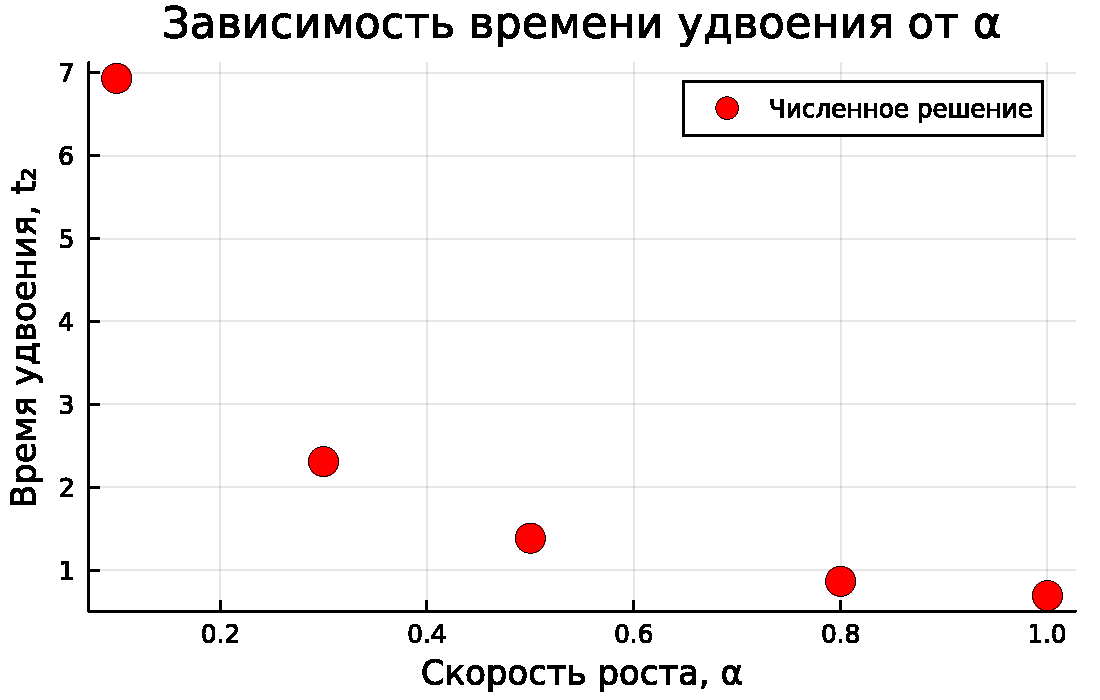
\includegraphics[keepaspectratio]{simulation-modeling-lab01-report_files/figure-pdf/cell-17-output-1.pdf}}

Теоретическая кривая: t₂ = ln(2)/α

\begin{Shaded}
\begin{Highlighting}[]
\NormalTok{α\_range }\OperatorTok{=} \FloatTok{0.1}\OperatorTok{:}\FloatTok{0.01}\OperatorTok{:}\FloatTok{1.0}
\FunctionTok{plot!}\NormalTok{(p3, α\_range, }\FunctionTok{log}\NormalTok{(}\FloatTok{2}\NormalTok{) }\OperatorTok{./}\NormalTok{ α\_range,}
\NormalTok{label}\OperatorTok{=}\StringTok{"Теория: t₂ = ln(2)/α"}\NormalTok{,}
\NormalTok{lw}\OperatorTok{=}\FloatTok{2}\NormalTok{,}
\NormalTok{linestyle}\OperatorTok{=:}\NormalTok{dash,}
\NormalTok{linecolor}\OperatorTok{=:}\NormalTok{blue}
\NormalTok{)}
\end{Highlighting}
\end{Shaded}

\pandocbounded{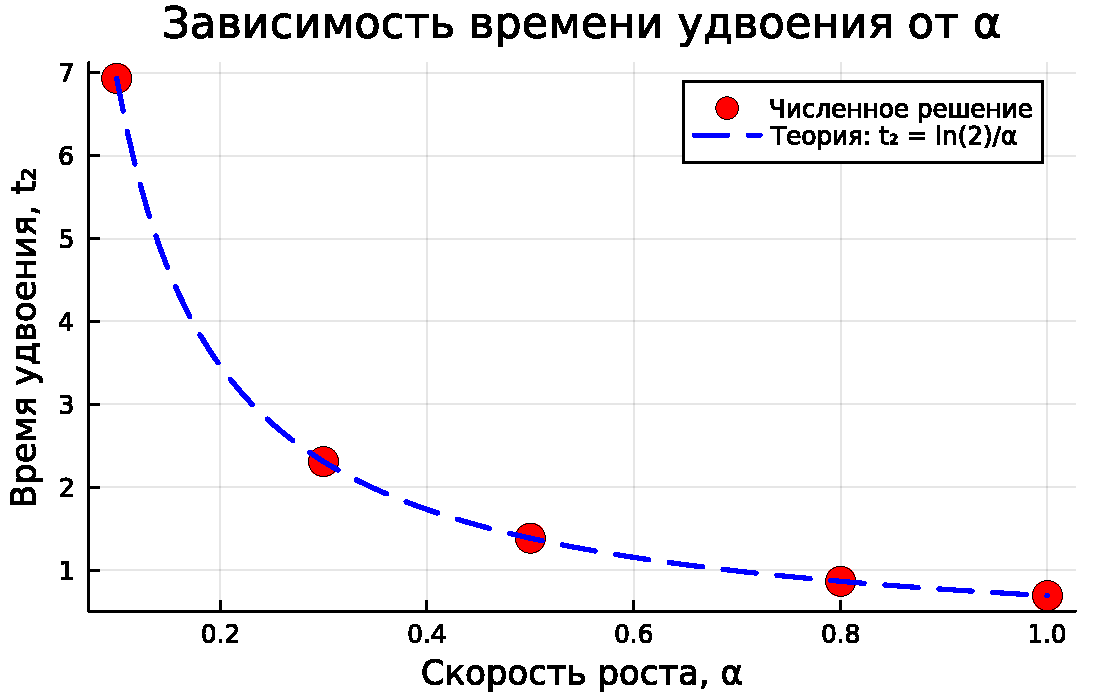
\includegraphics[keepaspectratio]{simulation-modeling-lab01-report_files/figure-pdf/cell-18-output-1.pdf}}

Сохраним график в папку plots

\begin{Shaded}
\begin{Highlighting}[]
\FunctionTok{savefig}\NormalTok{(}\FunctionTok{plotsdir}\NormalTok{(script\_name, }\StringTok{"doubling\_time\_vs\_alpha.png"}\NormalTok{))}
\end{Highlighting}
\end{Shaded}

\begin{verbatim}
"/home/svpavliuchenkov/work/study/2026-1/2026-1==study-simulation-modeling/2026-1--study--simulation--modeling/labs/lab01/project/plots/startup/doubling_time_vs_alpha.png"
\end{verbatim}

\section{Бенчмаркинг с разными
параметрами}\label{ux431ux435ux43dux447ux43cux430ux440ux43aux438ux43dux433-ux441-ux440ux430ux437ux43dux44bux43cux438-ux43fux430ux440ux430ux43cux435ux442ux440ux430ux43cux438}

\textbf{ИЗМЕНЕНИЕ:} Бенчмаркинг для разных значений α

\begin{Shaded}
\begin{Highlighting}[]
\FunctionTok{println}\NormalTok{(}\StringTok{"}\SpecialCharTok{\textbackslash{}n}\StringTok{"} \OperatorTok{*} \StringTok{"="}\OperatorTok{\^{}}\FloatTok{60}\NormalTok{)}
\FunctionTok{println}\NormalTok{(}\StringTok{"Бенчмаркинг для разных значений α"}\NormalTok{)}
\FunctionTok{println}\NormalTok{(}\StringTok{"="}\OperatorTok{\^{}}\FloatTok{60}\NormalTok{)}
\NormalTok{benchmark\_results }\OperatorTok{=}\NormalTok{ []}
\ControlFlowTok{for}\NormalTok{ α\_value }\KeywordTok{in}\NormalTok{ param\_grid[}\OperatorTok{:}\NormalTok{α]}
\NormalTok{bench\_params }\OperatorTok{=} \FunctionTok{Dict}\NormalTok{(}
\OperatorTok{:}\NormalTok{u0 }\OperatorTok{=\textgreater{}}\NormalTok{ [}\FloatTok{1.0}\NormalTok{],}
\OperatorTok{:}\NormalTok{α }\OperatorTok{=\textgreater{}}\NormalTok{ α\_value,}
\OperatorTok{:}\NormalTok{tspan }\OperatorTok{=\textgreater{}}\NormalTok{ (}\FloatTok{0.0}\NormalTok{, }\FloatTok{10.0}\NormalTok{),}
\OperatorTok{:}\NormalTok{solver }\OperatorTok{=\textgreater{}} \FunctionTok{Tsit5}\NormalTok{(),}
\OperatorTok{:}\NormalTok{saveat }\OperatorTok{=\textgreater{}} \FloatTok{0.1}
\NormalTok{) }\CommentTok{\# Подготавливаем параметры для бенчмарка}
\KeywordTok{function} \FunctionTok{benchmark\_run}\NormalTok{() }\CommentTok{\# Функция для бенчмарка}
\NormalTok{prob }\OperatorTok{=} \FunctionTok{ODEProblem}\NormalTok{(exponential\_growth!,}
\NormalTok{bench\_params[}\OperatorTok{:}\NormalTok{u0],}
\NormalTok{bench\_params[}\OperatorTok{:}\NormalTok{tspan],}
\NormalTok{(α}\OperatorTok{=}\NormalTok{bench\_params[}\OperatorTok{:}\NormalTok{α],))}
\ControlFlowTok{return} \FunctionTok{solve}\NormalTok{(prob, bench\_params[}\OperatorTok{:}\NormalTok{solver];}
\NormalTok{saveat}\OperatorTok{=}\NormalTok{bench\_params[}\OperatorTok{:}\NormalTok{saveat])}
\ControlFlowTok{end}
\FunctionTok{println}\NormalTok{(}\StringTok{"}\SpecialCharTok{\textbackslash{}n}\StringTok{Бенчмарк для α = }\SpecialCharTok{$}\StringTok{α}\NormalTok{\_value}\StringTok{:"}\NormalTok{)}
\NormalTok{b }\OperatorTok{=} \PreprocessorTok{@benchmark} \OperatorTok{$}\FunctionTok{benchmark\_run}\NormalTok{() samples}\OperatorTok{=}\FloatTok{100}\NormalTok{ evals}\OperatorTok{=}\FloatTok{1} \CommentTok{\# Запускбенчмарка↪}
\FunctionTok{push!}\NormalTok{(benchmark\_results, (α}\OperatorTok{=}\NormalTok{α\_value, time}\OperatorTok{=}\FunctionTok{median}\NormalTok{(b).time}\OperatorTok{/}\FloatTok{1e9}\NormalTok{)) }\CommentTok{\#время в секундах↪}
\FunctionTok{println}\NormalTok{(}\StringTok{" Среднее время: "}\NormalTok{, }\FunctionTok{round}\NormalTok{(}\FunctionTok{median}\NormalTok{(b).time}\OperatorTok{/}\FloatTok{1e9}\NormalTok{;digits}\OperatorTok{=}\FloatTok{4}\NormalTok{), }\StringTok{" сек"}\NormalTok{)}
\KeywordTok{end}
\end{Highlighting}
\end{Shaded}

\begin{verbatim}

============================================================
Бенчмаркинг для разных значений α
============================================================

Бенчмарк для α = 0.1:
 Среднее время: 0.0 сек

Бенчмарк для α = 0.3:
 Среднее время: 0.0 сек

Бенчмарк для α = 0.5:
 Среднее время: 0.0 сек

Бенчмарк для α = 0.8:
 Среднее время: 0.0 сек

Бенчмарк для α = 1.0:
 Среднее время: 0.0 сек
\end{verbatim}

График зависимости времени вычисления от α

\begin{Shaded}
\begin{Highlighting}[]
\NormalTok{bench\_df }\OperatorTok{=} \FunctionTok{DataFrame}\NormalTok{(benchmark\_results)}
\NormalTok{p4 }\OperatorTok{=} \FunctionTok{plot}\NormalTok{(bench\_df.α, bench\_df.time,}
\NormalTok{seriestype}\OperatorTok{=:}\NormalTok{scatter,}
\NormalTok{label}\OperatorTok{=}\StringTok{"Время вычисления"}\NormalTok{,}
\NormalTok{xlabel}\OperatorTok{=}\StringTok{"Скорость роста, α"}\NormalTok{,}
\NormalTok{ylabel}\OperatorTok{=}\StringTok{"Время вычисления, сек"}\NormalTok{,}
\NormalTok{title}\OperatorTok{=}\StringTok{"Зависимость времени вычисления от α"}\NormalTok{, markersize}\OperatorTok{=}\FloatTok{8}\NormalTok{,}
\NormalTok{markercolor}\OperatorTok{=:}\NormalTok{green,}
\NormalTok{legend}\OperatorTok{=:}\NormalTok{topleft}
\NormalTok{)}
\end{Highlighting}
\end{Shaded}

\pandocbounded{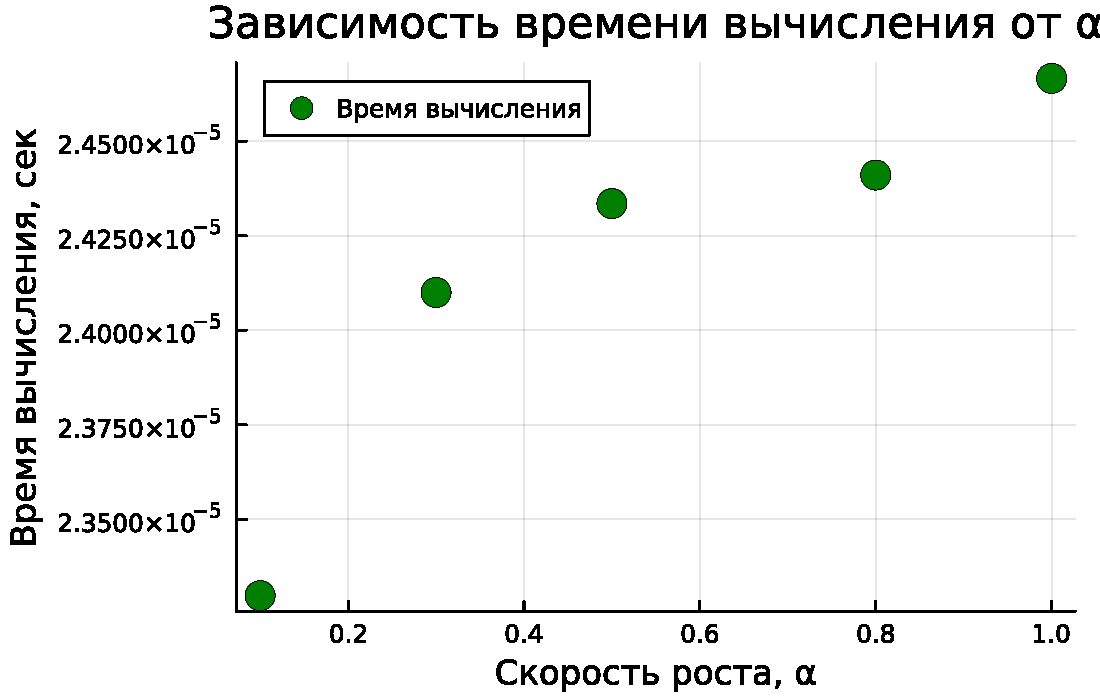
\includegraphics[keepaspectratio]{simulation-modeling-lab01-report_files/figure-pdf/cell-21-output-1.pdf}}

Сохраним график в папку plots

\begin{Shaded}
\begin{Highlighting}[]
\FunctionTok{savefig}\NormalTok{(}\FunctionTok{plotsdir}\NormalTok{(script\_name, }\StringTok{"computation\_time\_vs\_alpha.png"}\NormalTok{))}
\end{Highlighting}
\end{Shaded}

\begin{verbatim}
"/home/svpavliuchenkov/work/study/2026-1/2026-1==study-simulation-modeling/2026-1--study--simulation--modeling/labs/lab01/project/plots/startup/computation_time_vs_alpha.png"
\end{verbatim}

\section{Сохранение всех
результатов}\label{ux441ux43eux445ux440ux430ux43dux435ux43dux438ux435-ux432ux441ux435ux445-ux440ux435ux437ux443ux43bux44cux442ux430ux442ux43eux432}

\textbf{НОВАЯ СЕКЦИЯ:} Сохранение сводных данных для
последующегоанализа↪

\begin{Shaded}
\begin{Highlighting}[]
\PreprocessorTok{@save} \FunctionTok{datadir}\NormalTok{(script\_name, }\StringTok{"all\_results.jld2"}\NormalTok{) base\_params param\_grid all\_params results\_df bench\_df}
\PreprocessorTok{@save} \FunctionTok{datadir}\NormalTok{(script\_name, }\StringTok{"all\_plots.jld2"}\NormalTok{) p1 p2 p3 p4}
\FunctionTok{println}\NormalTok{(}\StringTok{"}\SpecialCharTok{\textbackslash{}n}\StringTok{"} \OperatorTok{*} \StringTok{"="}\OperatorTok{\^{}}\FloatTok{60}\NormalTok{)}
\FunctionTok{println}\NormalTok{(}\StringTok{"ЛАБОРАТОРНАЯ РАБОТА ЗАВЕРШЕНА"}\NormalTok{)}
\FunctionTok{println}\NormalTok{(}\StringTok{"="}\OperatorTok{\^{}}\FloatTok{60}\NormalTok{)}
\FunctionTok{println}\NormalTok{(}\StringTok{"}\SpecialCharTok{\textbackslash{}n}\StringTok{Результаты сохранены в:"}\NormalTok{)}
\FunctionTok{println}\NormalTok{(}\StringTok{" • data/}\SpecialCharTok{$}\NormalTok{(script\_name)}\StringTok{/single/ {-} базовыйэксперимент"}\NormalTok{)}
\FunctionTok{println}\NormalTok{(}\StringTok{" • data/}\SpecialCharTok{$}\NormalTok{(script\_name)}\StringTok{/parametric\_scan/ {-}параметрическое сканирование"}\NormalTok{)}
\FunctionTok{println}\NormalTok{(}\StringTok{" • data/}\SpecialCharTok{$}\NormalTok{(script\_name)}\StringTok{/all\_results.jld2 {-} сводныеданные"}\NormalTok{)}
\FunctionTok{println}\NormalTok{(}\StringTok{" • plots/}\SpecialCharTok{$}\NormalTok{(script\_name)}\StringTok{/ {-} все графики"}\NormalTok{)}
\FunctionTok{println}\NormalTok{(}\StringTok{" • data/}\SpecialCharTok{$}\NormalTok{(script\_name)}\StringTok{/all\_plots.jld2 {-} объектыграфиков"}\NormalTok{)}
\FunctionTok{println}\NormalTok{(}\StringTok{"}\SpecialCharTok{\textbackslash{}n}\StringTok{Для анализа результатов используйте:"}\NormalTok{)}
\FunctionTok{println}\NormalTok{(}\StringTok{" using JLD2, DataFrames"}\NormalTok{)}
\FunctionTok{println}\NormalTok{(}\StringTok{" @load }\SpecialCharTok{\textbackslash{}"}\StringTok{data/}\SpecialCharTok{$}\NormalTok{(script\_name)}\StringTok{/all\_results.jld2}\SpecialCharTok{\textbackslash{}"}\StringTok{"}\NormalTok{)}
\FunctionTok{println}\NormalTok{(}\StringTok{" println(results\_df)"}\NormalTok{)}
\end{Highlighting}
\end{Shaded}

\begin{verbatim}

============================================================
ЛАБОРАТОРНАЯ РАБОТА ЗАВЕРШЕНА
============================================================

Результаты сохранены в:
 • data/startup/single/ - базовыйэксперимент
 • data/startup/parametric_scan/ -параметрическое сканирование
 • data/startup/all_results.jld2 - сводныеданные
 • plots/startup/ - все графики
 • data/startup/all_plots.jld2 - объектыграфиков

Для анализа результатов используйте:
 using JLD2, DataFrames
 @load "data/startup/all_results.jld2"
 println(results_df)
\end{verbatim}

\chapter{Выводы}\label{ux432ux44bux432ux43eux434ux44b}

В ходе лабораторной работы было подготовлено рабочее пространство для
выполнения программ и приобретены необходимые навыки создания и
преобразования программ на Julia.


\printbibliography



\end{document}
